\documentclass[../Main.tex]{subfiles}

\begin{document}
\section{Basic Postulates of Relativity}
Maxwell's Equations, formulated by Maxwell in 1862, predict the existence of electromagnetic waves that travel at the speed of light. This is $c = 299792458 m s^{-1}$ (note that this number is precise, because it defines the metre).\par
A theory such as Maxwell's equations with a preferred velocity cannot be Galilean invariant. In principle this is permissible, sound waves travel through the air around $300 ms^{-1}$, but this is relative to the rest frame of the air. Thus, it was assumed that light must travel through a medium, this proposed medium was known as the Luminiferous Ether. However, experiments to demonstrate the existence of the Luminiferous Ether (Michelson \& Morley, 1881) showed that light travels at the same speed regardless of how fast the observer (on Earth) is moving through the Ether.\par
In 1905, Einstein postulated that there was no Ether. He provided two postulates:
\begin{enumerate}
    \item The laws of physics are the same in all inertial reference frames. This is the principle of relativity that Galileo postulated before.
    \item The speed of light in a vacuum is the same in all inertial reference frames. This is clearly not compatible with Galilean Relativity.
\end{enumerate}
\section{Lorentz Transformations in One Dimension}
\subsection{Deriving Lorentz Transformations}
We will derive the Lorentz transformations to replace Galilean transformations.\par
We will first consider 1 spatial dimension. An inertial frame $S$ has coordinates $(x, t)$. Consider a second frame $S'$ that moves at a speed $v$ relative to $S$ and has coordinates $(x', t')$.\par
According to Galileo, $x' = x - vt$ and $t' = t$.\par
This will not work, as the speed of light will not be constant in both frames. Instead consider a general transformation:
\begin{align*}
    x' &= f(x, t) \\
    t' &= g(x, t) \\
\end{align*}
Postulate 1 requires that in both frames $S$ and $S'$, a particle experiencing no forces must move at a constant velocity (Law of Inertia). So for a free particle in $S$, with $x = A + Bt$, the particle in $S'$ must be moving with $x' = A' + B't'$. Therefore the transformation $(f, g)$ must map lines in the $(x, t)$ plane to lines in the $(x', t')$ plane. Therefore $f$ and $g$ must be linear:
\begin{align*}
    x' &= ax + bt \\
    t' &= cx + dt
\end{align*}
Note that $a, b, c, d$ could depend on $v$ but must not depend on $x, t$. Note also that we have chosen the frames to have a common origin. We could just as well have added a constant term to both of the above equations.\par
The frame $S'$ is moving at speed $v$ in the frame $S$, but obviously must be at rest with respect to itself, $x' = 0$. Therefore the line $x = vt$ must be mapped to the line $x' = 0$. Therefore we can get the function $f$ up to scaling:
\begin{equation*}
    x' = \gamma_v (x - vt)
\end{equation*}
We can also relate in the other direction: $S$ moves at speed $-v$ in relation to $S'$, so $x = \gamma_{-v} (x' + vt)$.
\begin{proposition}
    In the above, $\gamma_v = \gamma_{-v}$
\end{proposition}
If we assume this to be true, we have that:
\begin{align}
    x' &= \gamma(x - vt) \label{eqnRelativePosGamma} \\
    t' &= \frac{1-\gamma^2}{\gamma v} x + \gamma t \label{eqnRelativeTimeGamma}
\end{align}
We cannot give a rigorous proof. We give 3 arguments:
\begin{enumerate}
    \item There is no preferred direction of space. Therefore $\gamma_v$ should be a function of $|v|$ only: $\gamma_v = \gamma_{-v}$.
    \item Consider frames $\tilde{S}$ and $\tilde{S'}$ where the $x$ axis is reflected. That is, $\tilde{x} = -x, \tilde{x'} = -x'$. Then if $S$ moves at speed $v$ with respect to $S'$, $\tilde{S}$ moves at speed $-v$ with respect to $\tilde{S'}$. Therefore
    \begin{align*}
        \tilde{x'} &= \gamma_{-v}(\tilde{x} + vt) \\
        -x' &= \gamma_{-v} (-x + vt) \\
        x' &= \gamma_{-v} (x - vt) \\
        \gamma_v &= \gamma_{-v}
    \end{align*}
    \item If a particle increases to speed $v$ relative to $S$, and then changes its speed by $-v$, it returns to rest is $S$. Consider the $x$ coordinate after these two changes in speed, assuming $\gamma_v = \gamma_{-v} = \gamma$:
        \begin{align*}
            x'' &= \gamma_{-v} (x' + vt') \\
            &= \gamma \left(\gamma (x - vt) + v\left(\gamma t + \frac{1 - \gamma^2}{\gamma v}\right)\right) \\
            &= x
        \end{align*}
\end{enumerate}
The final piece of information is postulate 2: the speed of light is the same in all frames. Therefore the light ray (path taken by light) $x = ct$ in $S$ must map to another light ray $x' = ct'$ under a Lorentz transformation.
\begin{align*}
    x' &= ct' \\
    \gamma (x - vt) &= c(\gamma t + \frac{1 - \gamma^2}{\gamma v}x) \\
    \gamma (c - v)t &= c(\gamma + \frac{1 - \gamma^2}{\gamma v}c)t \\
    \gamma (c - v) &= c(\gamma + \frac{1 - \gamma^2}{\gamma v}c)
\end{align*}
Then solving this final equation (a quadratic) for $\gamma$, the result is:
\begin{equation}
    \gamma = \frac{1}{\sqrt{1 - \frac{v^2}{c^2}}}
    \label{eqnLorentzFactor}
\end{equation}
Note that here we choose the positive root, since the negative root would correspond to a reflection in the axis.\par
Our equations \ref{eqnRelativePosGamma} and \ref{eqnRelativeTimeGamma} then become:
\begin{align}
    x' &= \gamma (x - vt) \label{eqnRelativePos} \\
    t' &= \gamma \left(t - \frac{v}{c^2}x\right) \label{eqnRelativeTime}
\end{align}
We can also check that in the case $v << c$ we recover Galilean Transformations: here we have $\gamma \approx 1$ and $\frac{v}{c} \approx 0$, and we do indeed get $x' = x - vt, t' = t$.
\subsection{Addition of Velocities}
We consider a particle moving with speed $u'$ in a frame $S'$, which in turn moves at speed $v$ in a frame $S$. We therefore consider what speed the particle moves in frame $S$.
\begin{equation*}
    u = \frac{x}{t}
\end{equation*}
We require the inverse Lorentz transformations. We have already argued that these are:
\begin{align*}
    x &= \gamma (x' + vt') \\
    t &= \gamma (t' + \frac{v}{c^2}x')
\end{align*}
\begin{align*}
    u &= \frac{x}{t} = \frac{\gamma(x' + vt')}{\gamma(t' + \frac{v}{c^2}x')} \\
    &= \frac{\frac{x'}{t'} + v}{1 + \frac{v}{c^2}\frac{x'}{t'}} \\
\end{align*}
\begin{equation}
    u = \frac{u' + v}{1 + \frac{vu'}{c^2}}
    \label{eqnAdditionVelocities}
\end{equation}
Again, note that this denominator is approximately 1 when $v$ and $u'$ are much smaller than $c$.
\begin{example}
    Consider, for example, $u' = v = \frac{c}{2}$. Then equation~\ref{eqnAdditionVelocities} gives that the added velocity is:
    \begin{equation*}
        u = \frac{c}{1 + \frac{1}{4}} = \frac{4}{5} c
    \end{equation*}
    Also, if one of the speeds is $c$: as in the case $v = c, u' = \frac{c}{d}$ where $d > 1$:
    \begin{align*}
        thing &= thing %TODO: Finish
    \end{align*}
\end{example}
Therefore, we cannot make something go faster than the speed of light by considering a frame moving towards it.
\subsection{Spacetime Diagrams and Simultaneity}
We introduce spacetime diagrams, an example of which is in figure~\ref{figSpacetimeDiagram}.
\begin{figure}[ht]
    \centering
    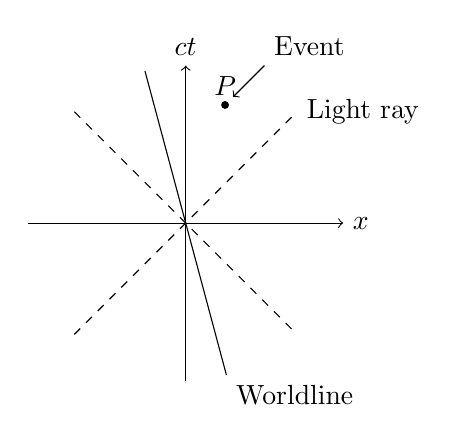
\begin{tikzpicture}
        \draw[->] (-2, 0) -- (2, 0) node[right] {$x$};
        \draw[->] (0, -2) -- (0, 2) node[above] {$ct$};

        \fill (0.5, 1.5) circle[radius=0.5mm];
        \node[anchor=south] at (0.5, 1.5) {$P$};

        \draw[->] (1, 2) node[anchor=south west] {Event} -- (0.6, 1.6);
        \draw[dashed] (225:2) -- (45:2) node[anchor=west] {Light ray};
        \draw[dashed] (135:2) -- (315:2);
        
        \draw (285:2) node[anchor=north west] {Worldline}
            -- (105:2);
    \end{tikzpicture}
    \caption{An example spacetime diagram}
    \label{figSpacetimeDiagram}
\end{figure}
We may put axes for a different frame $S'$ on the spacetime diagram of frame $S$. Let this move at speed $v$ relative to $S$. Then the $t'$ axis is when $x' = 0$, that is $ct = \frac{c}{v} x$. The $x'$ axis is at $t' = 0$, which is $ct = \frac{v}{c} x$. Figure~\ref{figSpacetimeDoubleAxis} shows what these new axes look like.
\begin{figure}[ht]
    \centering
    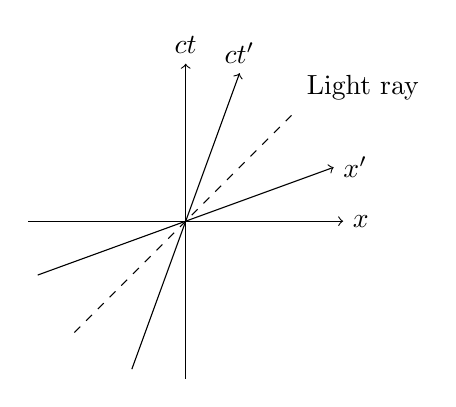
\begin{tikzpicture}
        \draw[->] (-2, 0) -- (2, 0) node[right] {$x$};
        \draw[->] (0, -2) -- (0, 2) node[above] {$ct$};
        \draw[->] (200:2) -- (20:2) node[right] {$x'$};
        \draw[->] (250:2) -- (70:2) node[above] {$ct'$};
        \draw[dashed] (225:2) -- (45:2) node[above right] {Light ray};
    \end{tikzpicture}
    \caption{Spacetime diagram with two sets of axes.}    
    \label{figSpacetimeDoubleAxis}
\end{figure}
Axes are always symmetric about the line $ct = x$, the path of a light ray.\par
We may also draw lines of constant $t$ or $t'$. These are horizontal in the frame $S$. Events that happen at the same time in the frame $S$ are \underline{simultaneous}. However, lines of constant $t'$ are not horizontal, so the same events (that are simultaneous in frame $S'$) are not simultaneous in the frame $S'$. If two events are separated in space and happen at the same time in $S$, they do not necessarily happen at the same time in a different frame $S'$.\par
This is the \underline{relativity of simultaneity}. This is an immediate consequence of the invariance of the speed of light.\par
\subsection{Causality and Light Cones}
Causality is the physical idea that causes must come before effects. If we have no simultaneity, is it therefore possible that causes could be seen after effects in some frame? This notion is solved by the fact that lines of simultaneity cannot make an angle of greater than $\frac{\pi}{4}$ because a frame can have relative velocity at most $c$ to another. This idea is made clearer by \underline{light cones}.
\begin{figure}[ht]
    \centering
    \begin{tikzpicture}[scale=2]
        \draw[->] (-0.5, 0) -- (2.1, 0) node[right] {$x$};
        \draw[->] (0, -0.5) -- (0, 2.1) node[above] {$ct$};

        \node[anchor=west] at (1, 1) {$P$};
        \fill (1, 1) circle[radius=0.2mm];
        \fill (1, 1.3) circle[radius=0.2mm];
        \node[anchor=west] at (1.5, 1.3) {$R$};
        \fill (1.5, 1.3) circle[radius=0.2mm];

        \draw[pattern=north east lines] (1, 1) -- (2, 2) -- (0, 2) -- cycle;
        \draw[pattern=north east lines] (0, 0) -- (2, 0) -- (1, 1) -- cycle;
        \node[anchor=west, shape=rectangle, fill=white, inner sep=0pt, outer sep=2pt] at (1, 1.3) {$Q$};
        \draw[->] (2, 1.5) node[anchor=west, align=left] {Future\\light cone}
            -- (1, 1.5);
        \draw[->] (2, 0.5) node[anchor=west, align=left] {Past\\light cone}
            -- (1, 0.5);
        
    \end{tikzpicture}
    \caption{Spacetime diagram with light cones}
    \label{figLightCones}
\end{figure}
Then, in figure~\ref{figLightCones}, $Q$ could be caused by $P$, but $R$ could not be caused by $P$ since it is outside the future light cone. $P$ can be caused by any event inside the past light cone.
\end{document}